\documentclass[10pt, aspectratio=169]{beamer}

% --- Configuración de Idioma y Fuentes ---
\usepackage[utf8]{inputenc}
\usepackage[spanish]{babel}
\usepackage[T1]{fontenc}
\usepackage{helvet} 

% --- Paquetes Adicionales ---
\usepackage{graphicx}
\usepackage{booktabs}
\usepackage{tikz}
\usetikzlibrary{positioning}
\usepackage{xcolor}
\usepackage{amsmath}
\usepackage{amssymb}
\usepackage{appendixnumberbeamer}
\usepackage{multirow}
\usepackage{bookmark}

% --- Rutas de imágenes ---
\graphicspath{{../../results/figures/analysis/}}

% --- Definición de Colores IPA27 ---
\definecolor{brandgreen}{HTML}{007932}
\definecolor{softgreen}{HTML}{E8F5E9}
\definecolor{darkgrey}{HTML}{333333}
\definecolor{lightgrey}{HTML}{F5F5F5}
\definecolor{brandgreenlight}{HTML}{B2D8C1} % Para el rule de la portada

% --- Estilo de Beamer Personalizado ---
\usetheme{Boadilla}
\usecolortheme{default}
\setbeamertemplate{navigation symbols}{} 
\setbeamertemplate{items}[circle]        
\setbeamertemplate{sections/subsections in toc}[circle]

\setbeamercolor{palette primary}{bg=brandgreen, fg=white}
\setbeamercolor{palette secondary}{bg=brandgreen!80, fg=white}
\setbeamercolor{palette tertiary}{bg=brandgreen!60, fg=white}
\setbeamercolor{structure}{fg=brandgreen}
\setbeamercolor{title}{fg=brandgreen, bg=white}
\setbeamercolor{frametitle}{fg=brandgreen, bg=white}
\setbeamercolor{block title}{bg=brandgreen, fg=white}
\setbeamercolor{block body}{bg=softgreen, fg=black}

% Ajuste de pie de página simplificado
\setbeamertemplate{footline}{
  \leavevmode%
  \hbox{%
  \begin{beamercolorbox}[wd=.3333\paperwidth, left]{author in head/foot}%
    \hspace*{2ex}IPA27 Project - Metodología Detallada
  \end{beamercolorbox}%
  \begin{beamercolorbox}[wd=.3333\paperwidth, center]{title in head/foot}%
    \insertshorttitle
  \end{beamercolorbox}%
  \begin{beamercolorbox}[wd=.3333\paperwidth, right]{date in head/foot}%
    \insertframenumber{} / \inserttotalframenumber\hspace*{2ex} 
  \end{beamercolorbox}}%
  \vskip0pt%
}

% --- Logotipo ---
\logo{
\includegraphics[width=1cm]{logo_fa27.png}}

\title[IPA27]{Índice de Prosperidad Andaluz (IPA27)}
\subtitle{Arquitectura Técnica, Metodología de Armonización y Resultados (2016-2025)}
\author[Equipo IPA27]{Fundación Andalucía 27}
\date{\today}

\begin{document}

% --- Slide de Título Premium ---
{
\setbeamertemplate{footline}{} 
\begin{frame}[plain]
    \begin{tikzpicture}[remember picture, overlay]
        % Sidebar verde premium
        \fill[brandgreen] (current page.north west) rectangle ([xshift=4.5cm]current page.south west);
        
        % Logo Blanco
        \node[anchor=north] at ([xshift=2.25cm, yshift=-1.5cm]current page.north west) {
            
\includegraphics[width=3cm]{logo_fa27_white.png}
        };
        
        % Bloque de Título
        \node[anchor=north west, xshift=5.5cm, yshift=-2.5cm] at (current page.north west) {
            \begin{minipage}{0.65\paperwidth}
                {\fontsize{64}{74}\selectfont \textbf{\textcolor{brandgreen}{IPA27}}} \\[0.3cm]
                {\fontsize{26}{32}\selectfont \textcolor{darkgrey}{Índice de Prosperidad Andaluz}} \\[1.5cm]
                {\color{brandgreenlight}\rule{8cm}{4pt}} \\[0.8cm]
                {\Large \textcolor{darkgrey}{\textbf{Arquitectura Técnica, Metodología de Armonización} \\ y Análisis de Resultados (2016-2025)}}
            \end{minipage}
        };
        
        \node[anchor=south east, xshift=-1cm, yshift=1cm] at (current page.south east) {
            \begin{minipage}{0.4\paperwidth}
                \raggedleft
                {\Large \textbf{\textcolor{brandgreen}{Fundación Andalucía 27}}} \\
                \vspace{0.1cm}
                \textcolor{darkgrey}{\today}
            \end{minipage}
        };
    \end{tikzpicture}
\end{frame}
}

% --- 1. INTRODUCCIÓN ---
\section{Introducción}

{
\setbeamercolor{background canvas}{bg=brandgreen}
\begin{frame}[plain]
    \centering
    \vfill
    {\Huge\bfseries\color{white} I. INTRODUCCIÓN}\\[0.6cm]
    {\color{white}\rule{6cm}{2.5pt}}\\[1.5cm]
    
\includegraphics[width=2.5cm]{logo_fa27_white.png}
    \vfill
\end{frame}
}

\begin{frame}{Gobernanza y Rigor Técnico}
    \textbf{\textcolor{brandgreen}{Dirección Técnica}}
    \begin{itemize}
        \item \textbf{Manuel Alejandro Hidalgo}: Director Técnico. Profesor de Economía Aplicada. Responsable del diseño metodológico y supervisión del índice.
    \end{itemize}
    
    \vspace{0.6cm}
    
    \textbf{\textcolor{brandgreen}{Consejo Técnico Asesor}}
    \begin{itemize}
        \small
        \item \textbf{Rafael Doménech}: BBVA Research. Especialista en análisis económico y financiero.
        \item \textbf{Olga Cantó}: Universidad de Alcalá de Henares (UAH). Economía pública.
        \item \textbf{Antonio Villar}: Universidad Pablo de Olavide e IVIE. Economía regional.
        \item \textbf{Miguel Ángel García}: Universidad Rey Juan Carlos (URJC). Economía aplicada.
        \item \textbf{Lucía Gorjón}: ISEAK. Investigación socioeconómica de impacto.
    \end{itemize}
    
    \vfill
    \centering
    \footnotesize \textit{Misión del Consejo: Garantizar la independencia y el rigor técnico en cada ciclo de actualización del IPA27.}
\end{frame}

\begin{frame}{El paradigma de la Prosperidad en el Siglo XXI}
    \begin{columns}
        \begin{column}{0.6\textwidth}
            \textbf{Más allá del PIB: El consenso internacional}
            \begin{itemize}
                \item \textit{Informe Stiglitz-Sen-Fitoussi (2009)}: Necesidad de medir el bienestar real y la sostenibilidad.
                \item \textbf{Alineación con los ODS}: No dejar a nadie atrás.
            \end{itemize}
            \vspace{0.4cm}
            \textbf{Misión del IPA27}
            \begin{itemize}
                \item Medir el progreso sistémico de Andalucía.
                \item Proporcionar una herramienta de \textbf{monitorización trimestral} (no anual).
                \item Comparar frente al conjunto nacional y el resto de regiones españolas (CC.AA.).
            \end{itemize}
        \end{column}
        \begin{column}{0.4\textwidth}
            \begin{block}{Definición de Prosperidad}
                No solo crecimiento económico, sino la capacidad de una sociedad para generar oportunidades de bienestar, seguridad y libertad de forma sostenible en el tiempo.
            \end{block}
        \end{column}
    \end{columns}
\end{frame}

% Resto del documento... (lo mantendré igual pero fixeado)
% --- 2. ARQUITECTURA ---
\section{Arquitectura}
{
\setbeamercolor{background canvas}{bg=brandgreen}
\begin{frame}[plain]
    \centering
    \vfill
    {\Huge\bfseries\color{white} II. ARQUITECTURA TÉCNICA}\\[0.6cm]
    {\color{white}\rule{8cm}{2.5pt}}\\[1.5cm]
    
\includegraphics[width=2.5cm]{logo_fa27_white.png}
    \vfill
\end{frame}
}

\begin{frame}{Pilares y Dominios: La estructura del IPA27}
    \centering
    
\includegraphics[width=0.85\textwidth]{ipa27_brechas_dominios.png}
    \vfill
    \begin{itemize}
        \item \textbf{3 Dominios}: Economías Abiertas, Sociedades Inclusivas y Condiciones de Vida.
        \item \textbf{9 Pilares}: Desde Conocimiento e Inversión hasta Salud y Seguridad.
        \item \textbf{24 Indicadores}: Armonizados y normalizados (Z-score corregido).
    \end{itemize}
\end{frame}

% --- 3. METODOLOGÍA ---
\section{Metodología}
{
\setbeamercolor{background canvas}{bg=brandgreen}
\begin{frame}[plain]
    \centering
    \vfill
    {\Huge\bfseries\color{white} III. METODOLOGÍA DE ARMONIZACIÓN}\\[0.6cm]
    {\color{white}\rule{10cm}{2.5pt}}\\[1.5cm]
    
\includegraphics[width=2.5cm]{logo_fa27_white.png}
    \vfill
\end{frame}
}

% --- 4. RESULTADOS ---
\section{Resultados}
{
\setbeamercolor{background canvas}{bg=brandgreen}
\begin{frame}[plain]
    \centering
    \vfill
    {\Huge\bfseries\color{white} IV. ANÁLISIS DE RESULTADOS}\\[0.6cm]
    {\color{white}\rule{8cm}{2.5pt}}\\[1.5cm]
    
\includegraphics[width=2.5cm]{logo_fa27_white.png}
    \vfill
\end{frame}
}

\begin{frame}{Waterfall: Anatomía de la Brecha IPA27}
    \small
    \centering
    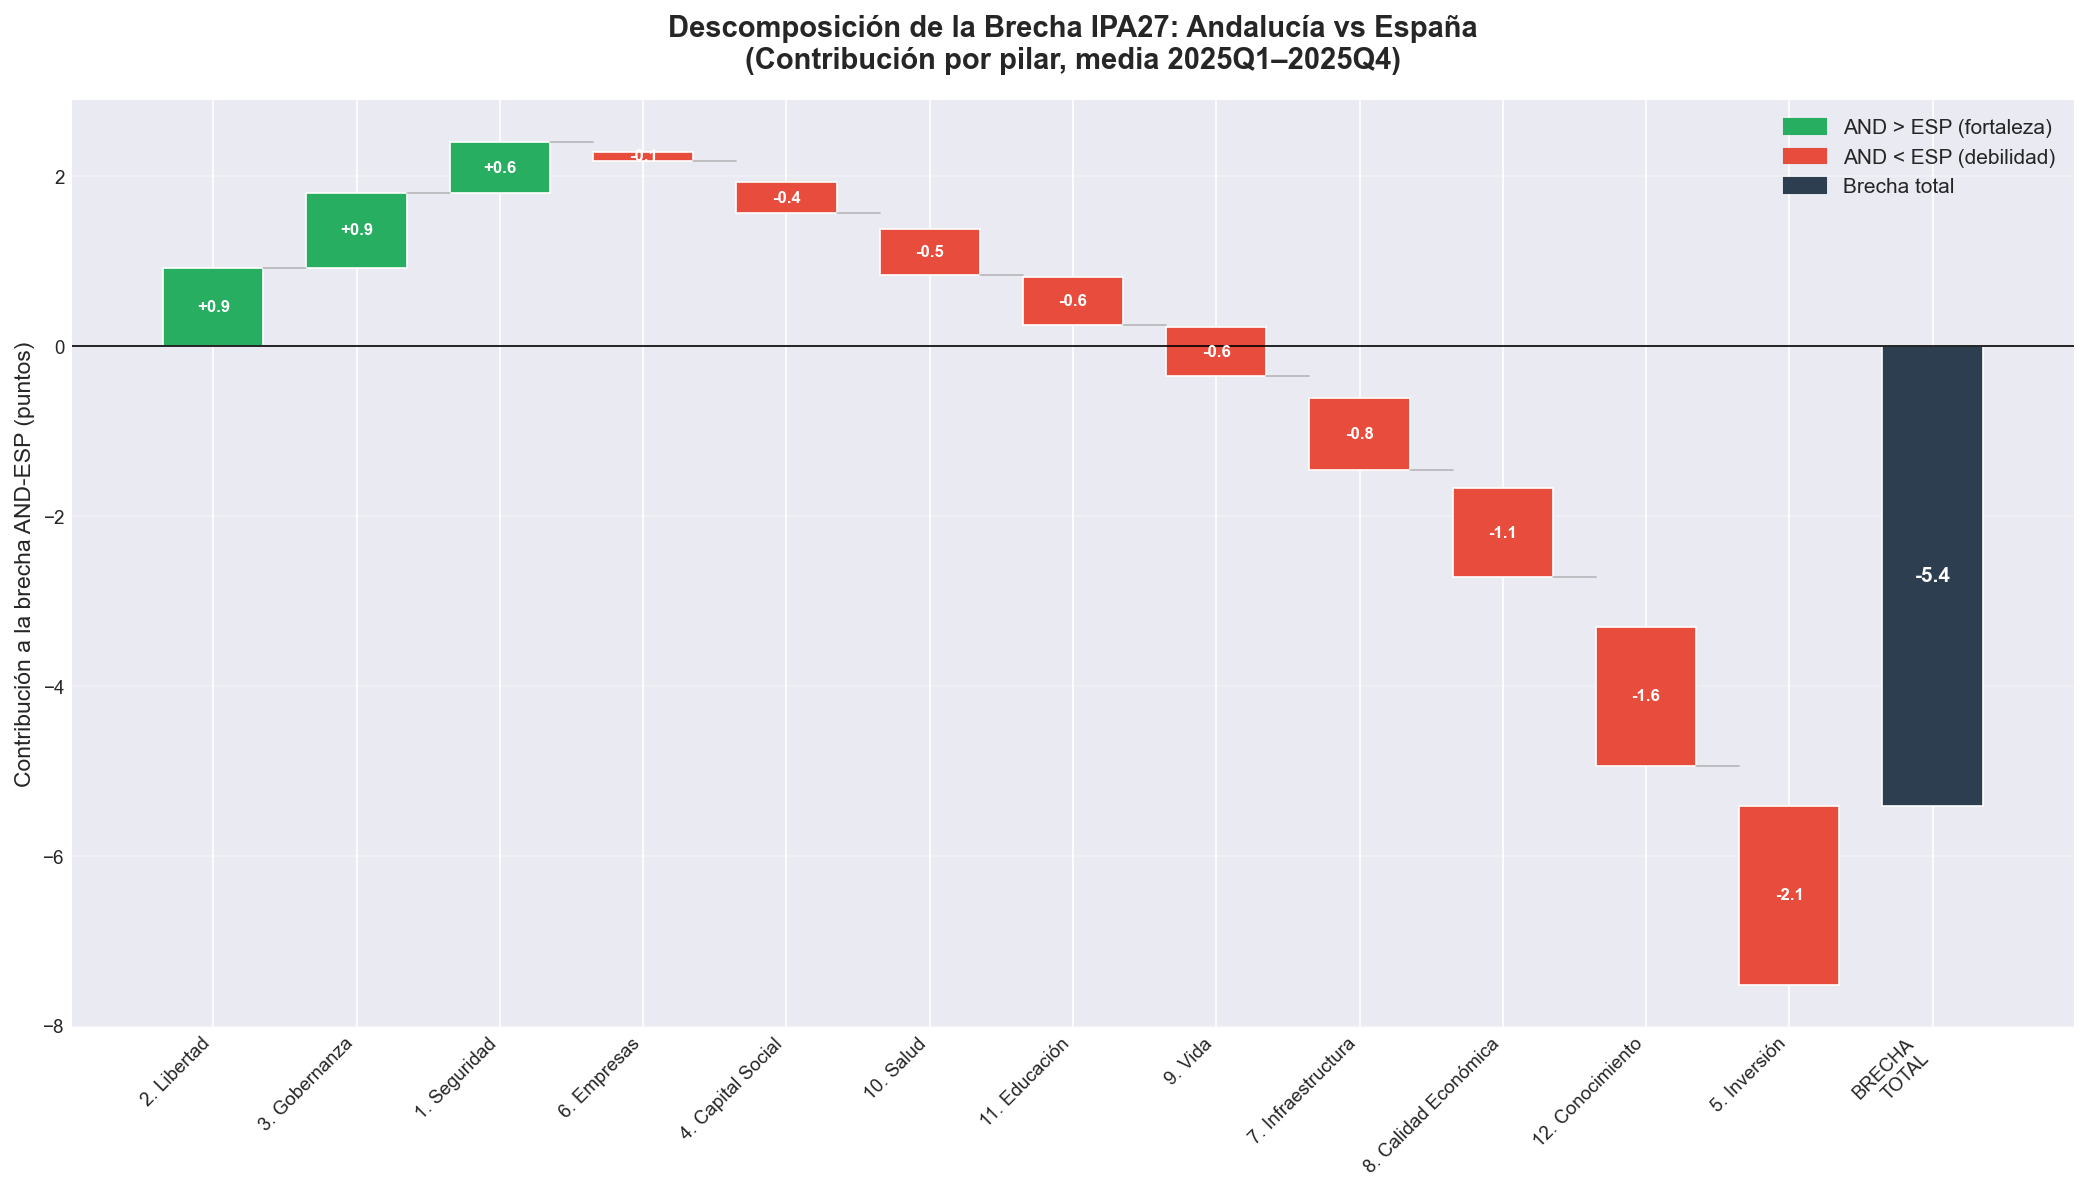
\includegraphics[width=0.7\textwidth]{ipa27_waterfall_brecha.png}
    \vfill
    \begin{itemize}
        \item \textbf{Brecha neta de -5.4 puntos} frente a la media nacional (2025Q4).
        \item \textbf{Fortalezas}: Libertad (+0.9), Gobernanza (+0.9) y Seguridad (+0.6).
        \item \textbf{Debilidades estructurales}: Inversión (-2.1), Conocimiento (-1.6).
    \end{itemize}
\end{frame}

\begin{frame}{Posición de Andalucía en la Distribución Regional}
    \centering
    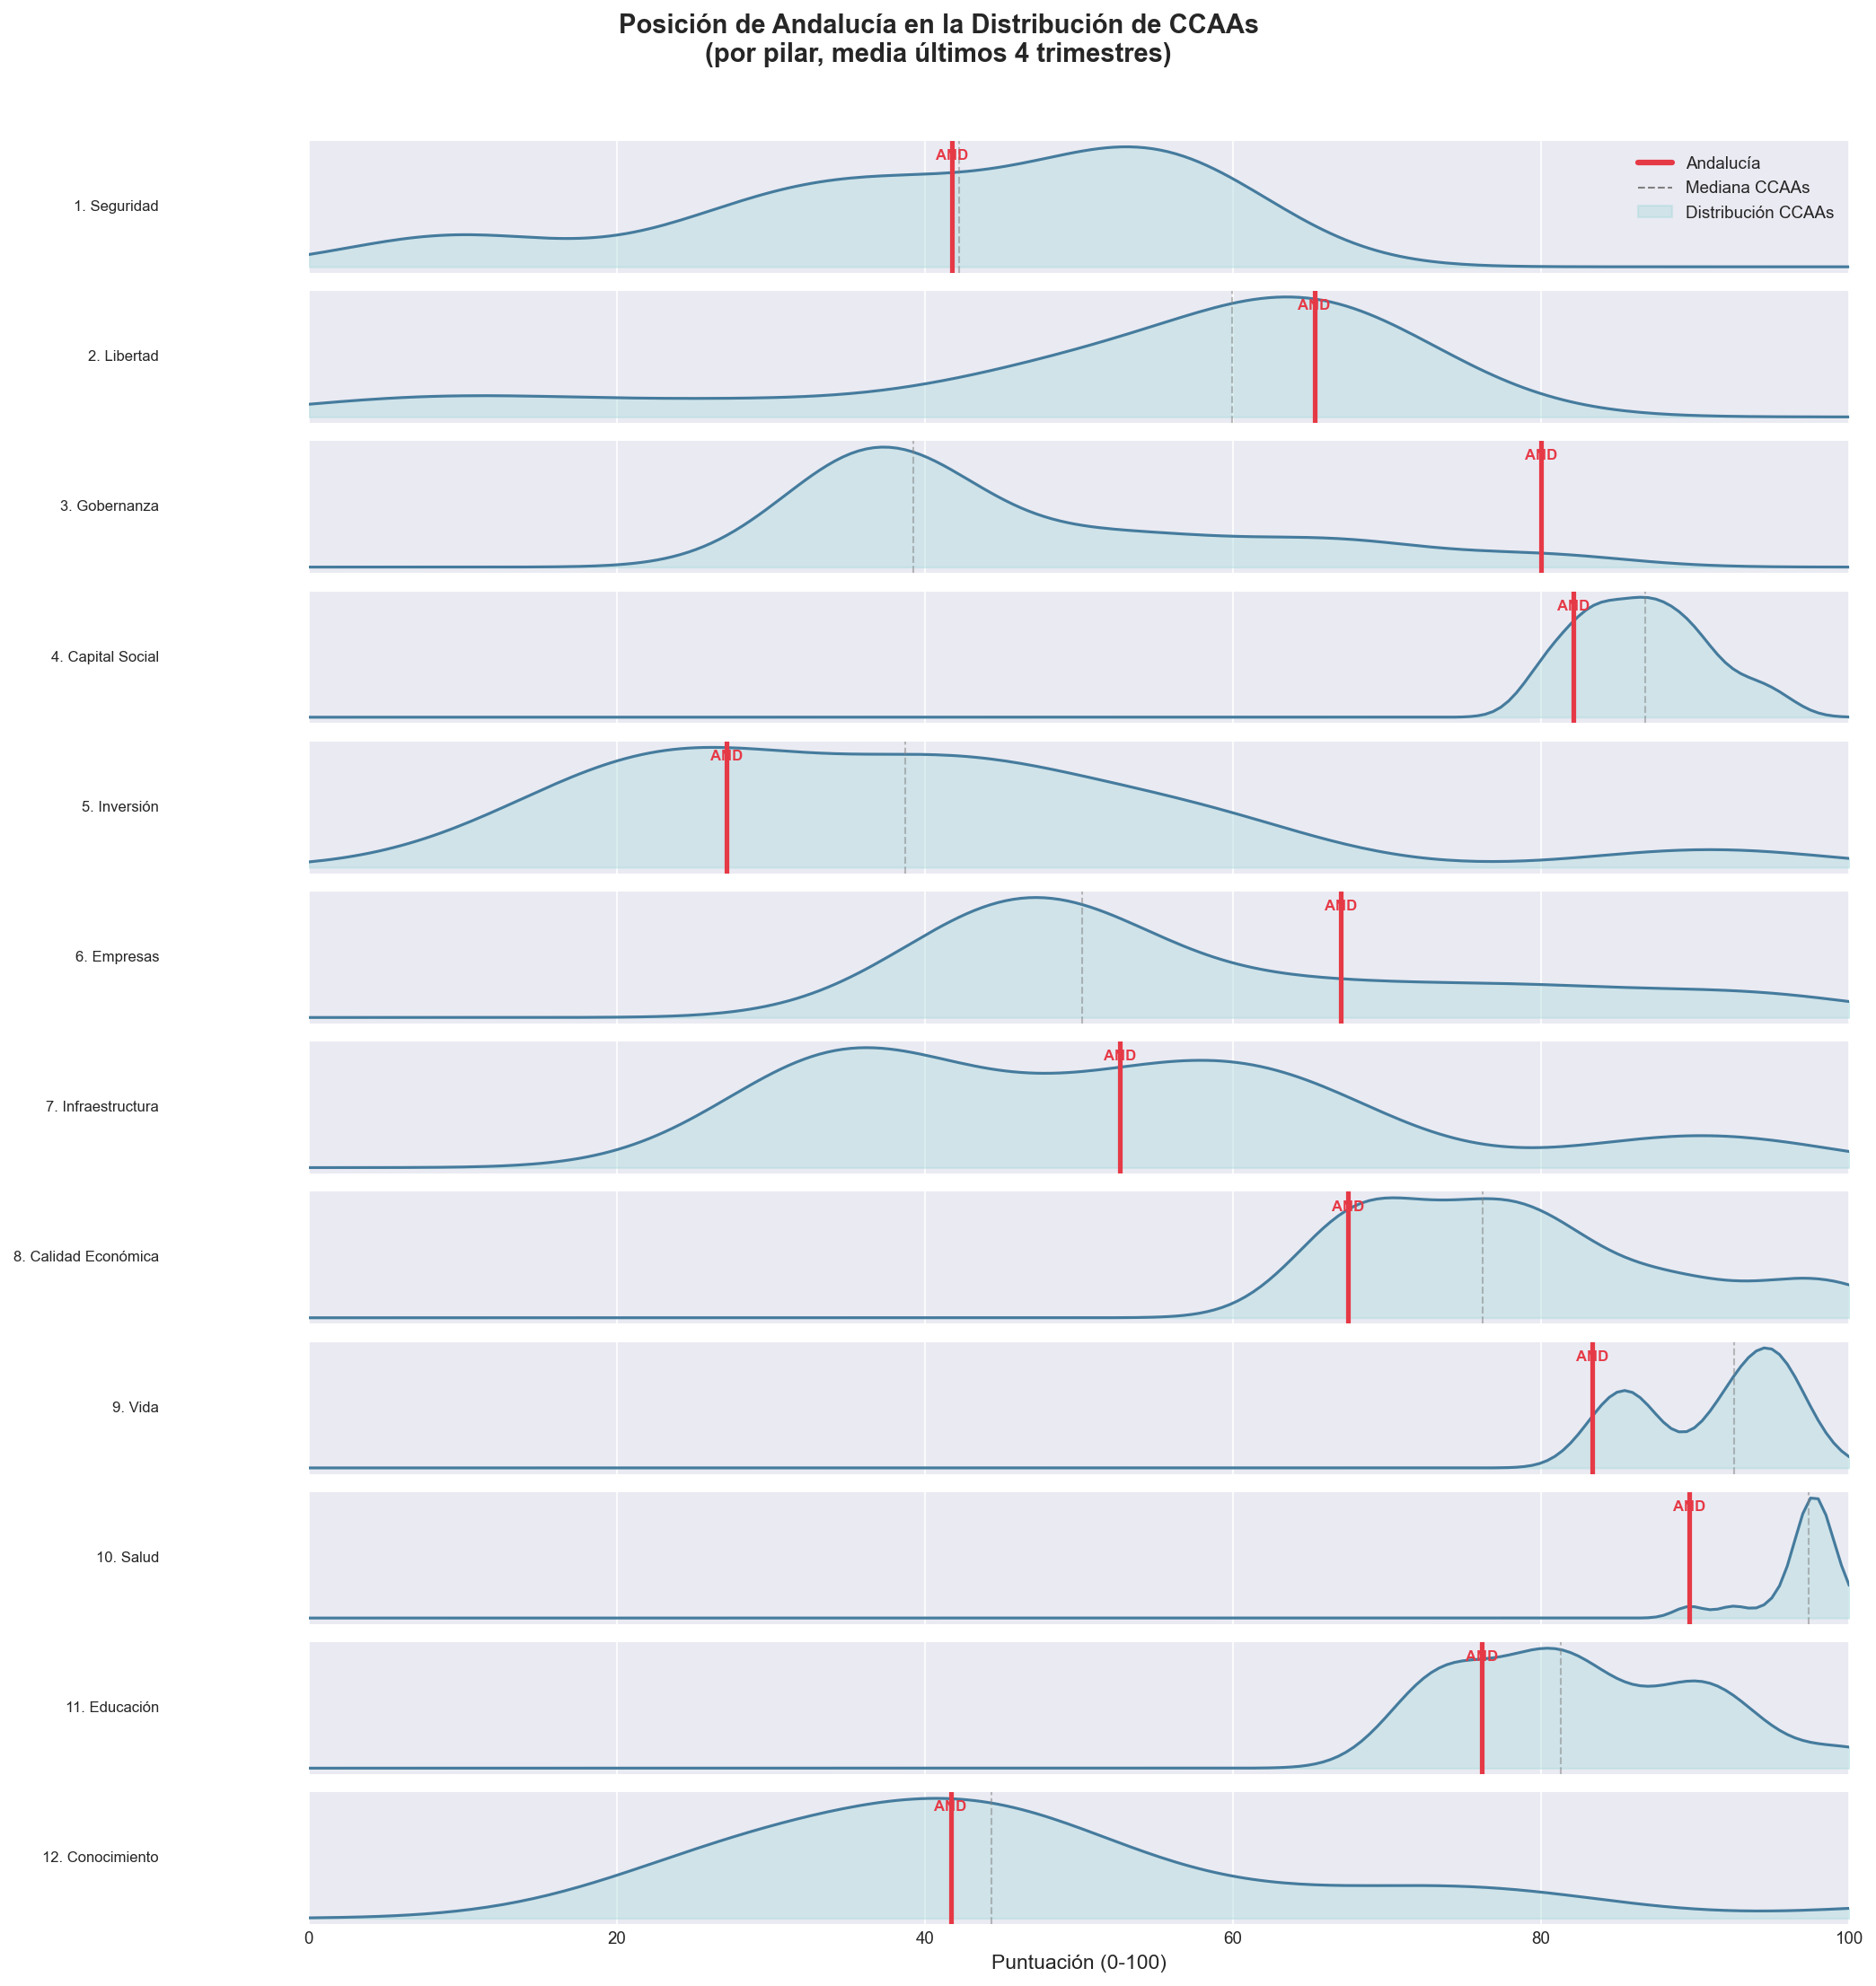
\includegraphics[width=0.7\linewidth]{ipa27_ridgeline_pilares.png}
    \vfill
    \begin{itemize}
        \item \textbf{Ridgeline Analysis}: Distribución de las 17 CCAA para cada pilar.
        \item Andalucía destaca positivamente en \textbf{Libertad} y \textbf{Gobernanza}.
    \end{itemize}
\end{frame}

% --- 5. AUDITORÍA ---
\section{Auditoría}
{
\setbeamercolor{background canvas}{bg=brandgreen}
\begin{frame}[plain]
    \centering
    \vfill
    {\Huge\bfseries\color{white} V. AUDITORÍA Y CALIDAD}\\[0.6cm]
    {\color{white}\rule{8cm}{2.5pt}}\\[1.5cm]
    
\includegraphics[width=2.5cm]{logo_fa27_white.png}
    \vfill
\end{frame}
}

\begin{frame}{Gracias por su atención}
    \centering
    \vfill
    {\Large \textbf{\textcolor{brandgreen}{Proyecto IPA27: Índice de Prosperidad Andaluz}}} \\
    \vspace{0.5cm}
    Fundación Andalucía 27 \\
    \today
    \vfill
\end{frame}

\end{document}
